\documentclass[aspectratio=169, table]{beamer}


%\usepackage[beamertheme=./praditatheme]{Pradita}

\usetheme{Pradita}

\title{Chapter-11:\\Orchestration-driven\\Service-oriented Architecture}
\subtitle{IF231303-Software Architecture}
\author{\textbf{Hansel Ricardo, Jonathan Erik, Yefta Tanuwijaya
        \\Alfa Yohannis}}
\begin{document}

	\begin{frame}[plain]
		\maketitle
	\end{frame}

   \section{Pendahuluan}
   \begin{frame}{Pendahuluan}
       \begin{itemize}
           \item Arsitektur Berorientasi Layanan (SOA) adalah pola arsitektur yang memungkinkan komponen-komponen perangkat lunak berkomunikasi satu sama lain melalui jaringan.
           \item SOA yang Dikendalikan Orkestrasi menekankan peran sentral orkestrasi dalam mengelola interaksi antara layanan-layanan.
       \end{itemize}
   \end{frame}

   \section{Arsitektur}
   \begin{frame}{Arsitektur}
       \begin{itemize}
           \item \textbf{Komponen}:
           \begin{itemize}
               \item Layanan Bisnis
               \item Bus Layanan Perusahaan (Mesin Orkestrasi, Pusat Integrasi)
               \item Layanan Perusahaan
               \item Layanan Aplikasi
               \item Layanan Infrastruktur
           \end{itemize}
       \end{itemize}
   \end{frame}

   \section{Sejarah}
   \begin{frame}{Sejarah}
       \begin{itemize}
           \item SOA yang Dikendalikan Orkestrasi berkembang dari kebutuhan akan sistem-sistem yang fleksibel dan dapat diskalakan untuk mendukung proses bisnis yang kompleks.
           \item Ini membangun pada prinsip-prinsip SOA tradisional tetapi menempatkan lebih banyak penekanan pada orkestrasi sebagai mekanisme kontrol sentral.
       \end{itemize}
   \end{frame}

   \section{Layanan Berbasis Orkestrasi}
   %        \framesubtitle{}
   \begin{frame}{Layanan Berbasis Orkestrasi}
       \vspace{30pt}
       \centering
       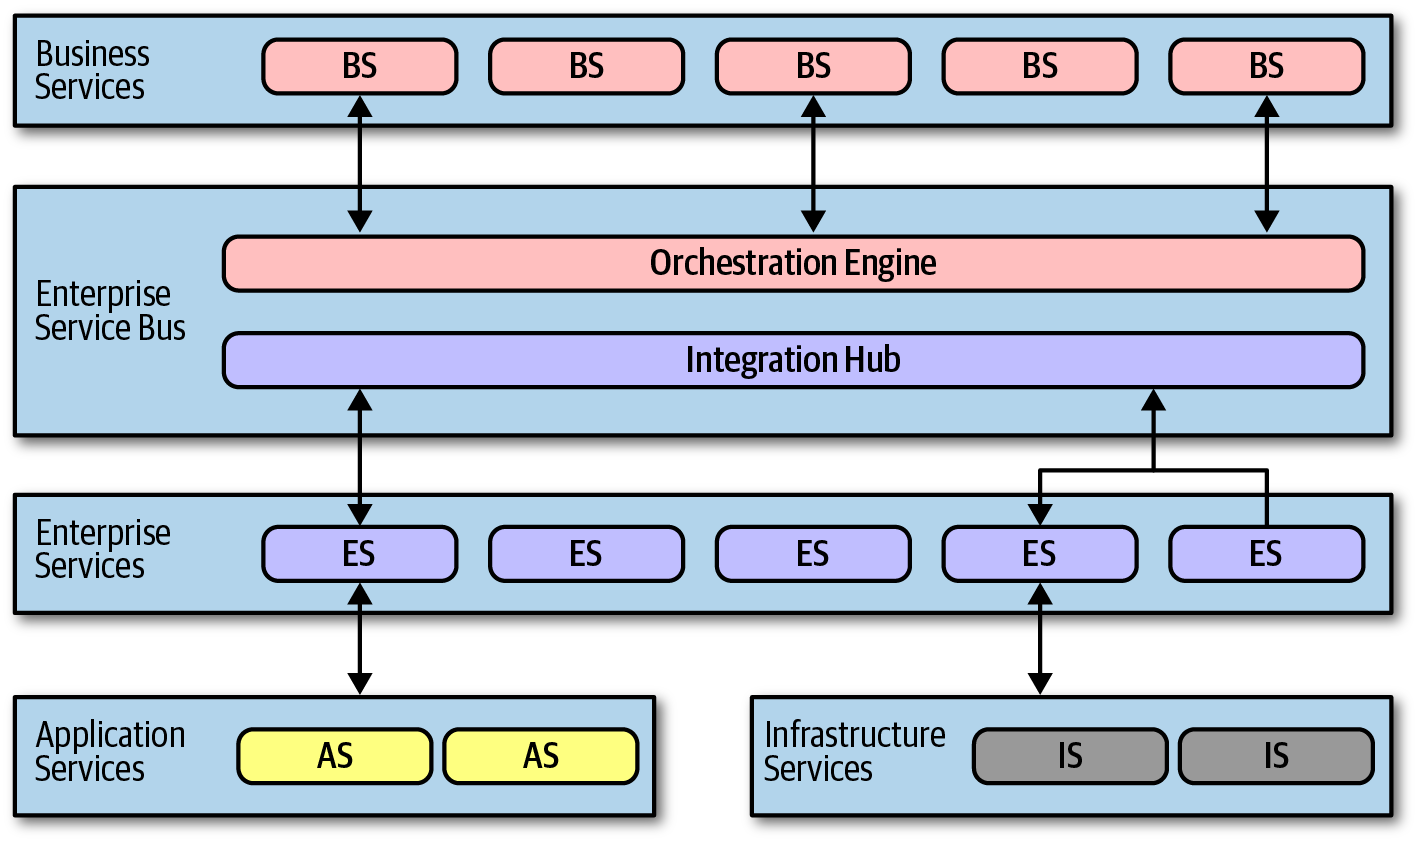
\includegraphics[width=0.8\textwidth]{../../images/orchestration-example}
   \end{frame}

   \section{Komponen}
   \begin{frame}{Komponen (1)}
       \begin{itemize}
           \item \textbf{Layanan Bisnis}: Mewakili fungsi inti domain bisnis. Contoh: Layanan manajemen pelanggan dalam platform e-commerce.
           \item \textbf{Bus Layanan Perusahaan (ESB)}:
           \begin{itemize}
               \item \textbf{Mesin Orkestrasi}: Mengkoordinasikan interaksi antara layanan berdasarkan alur kerja yang telah ditentukan sebelumnya. Contoh: Alur kerja pemrosesan pesanan dalam sistem ritel online.
               \item \textbf{Pusat Integrasi}: Mengelola konektivitas dan integrasi antara sistem dan aplikasi yang berbeda. Contoh: Integrasi sistem CRM, ERP, dan billing dalam sebuah perusahaan.
           \end{itemize}
       \end{itemize}
   \end{frame}

   \section{Komponen}
   \begin{frame}{Komponen (2)}
       \begin{itemize}
           \item \textbf{Layanan Perusahaan}: Layanan bersama yang menyediakan fungsionalitas umum di seluruh perusahaan. Contoh: Layanan otentikasi yang Dikendalikan oleh beberapa aplikasi dalam sebuah organisasi.
           \item \textbf{Layanan Aplikasi}: Layanan khusus untuk aplikasi atau proses bisnis tertentu. Contoh: Layanan pemrosesan pembayaran dalam aplikasi perbankan online.
           \item \textbf{Layanan Infrastruktur}: Layanan dasar seperti keamanan, logging, dan pemantauan.
       \end{itemize}
   \end{frame}

   \section{Keuntungan}
   \begin{frame}{Keuntungan}
       \begin{itemize}
           \item \textbf{Fleksibilitas}: Memungkinkan komposisi dan orkestrasi layanan secara dinamis untuk mendukung perubahan kebutuhan bisnis.
           \item \textbf{Skalabilitas}: Memungkinkan peningkatan layanan secara independen, menghasilkan penggunaan sumber daya yang lebih baik.
           \item \textbf{Interoperabilitas}: Memfasilitasi integrasi yang mulus antara sistem dan teknologi yang heterogen.
           \item \textbf{Kemungkinan Dikendalikan Kembali}: Mendorong penggunaan kembali layanan di beberapa aplikasi dan proses, mengurangi waktu dan usaha pengembangan.
       \end{itemize}
   \end{frame}

   \section{Kerugian}
   \begin{frame}{Kerugian}
       \begin{itemize}
           \item \textbf{Kompleksitas}: Mengelola logika orkestrasi dan koordinasi antara layanan dapat menjadi kompleks, terutama dalam implementasi besar.
           \item \textbf{Beban Kinerja}: Orkestrasi memperkenalkan beban pemrosesan tambahan, yang dapat mempengaruhi kinerja sistem.
           \item \textbf{Ketergantungan pada ESB}: Peran sentral Bus Layanan Perusahaan menciptakan titik kegagalan tunggal dan dapat menyebabkan ketergantungan pada vendor.
       \end{itemize}
   \end{frame}

   \section{Aplikasi/Contoh}
   \begin{frame}{Aplikasi/Contoh}
       \begin{itemize}
           \item \textbf{Manajemen Rantai Pasokan}: SOA yang Dikendalikan Orkestrasi umumnya Dikendalikan untuk menyederhanakan dan mengotomatiskan proses rantai pasokan yang melibatkan banyak pemangku kepentingan.
           \item \textbf{Layanan Keuangan}: Bank dan lembaga keuangan menggunakan SOA untuk mengintegrasikan sistem-sistem yang berbeda untuk transaksi, manajemen risiko, dan layanan pelanggan.
       \end{itemize}
   \end{frame}

   \section{Kesimpulan}
   \begin{frame}{Kesimpulan}
       \begin{itemize}
           \item SOA yang Dikendalikan Orkestrasi menawarkan kerangka kerja yang cocok untuk membangun sistem yang fleksibel, dapat diskalakan, dan interoperabel.
           \item Meskipun memiliki keuntungan seperti fleksibilitas dan skalabilitas, SOA yang Dikendalikan Orkestrasi juga memiliki tantangan dalam hal kompleksitas dan beban kinerja.
           \item Aplikasi dunia nyata di berbagai industri menunjukkan manfaat praktis SOA yang Dikendalikan Orkestrasi dalam mengoptimalkan proses bisnis dan meningkatkan efisiensi operasional.
       \end{itemize}
   \end{frame}




%	\begin{frame}{DevOps}
%		\begin{figure}[h]
%			\centering
%			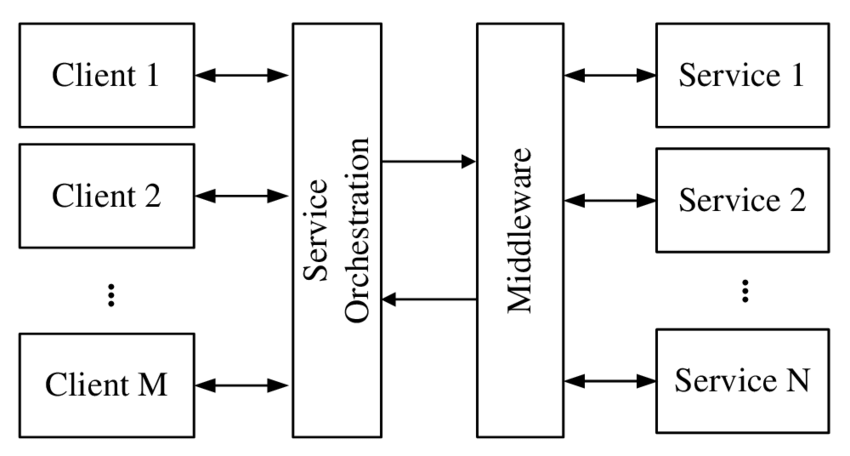
\includegraphics[width=\textwidth]{ODSOA}
%			\caption{Arsitektur ODSOA.}
%			\label{fig:Arsitektur ODSOA}
%		\end{figure}
%	\end{frame}
%
%	\begin{frame}{Latar Belakang}
%		\begin{itemize}
%			\item Pengertian
%			\\\textit{Orchestration-driven Service-oriented Architecture} (ODSOA) adalah suatu pendekatan arsitektur perangkat lunak yang bertujuan untuk memfasilitasi pengembangan dan integrasi sistem yang kompleks dengan cara menggunakan layanan (\textit{Services}) yang terdistribusi dan terpisah secara fisik namun saling terkait secara fungsional.
%		\end{itemize}
%	\end{frame}
%
%	\begin{frame}{Komponen}
%		Komponen utama dalam \textit{Orchestration-driven Service-oriented Architecture} (ODSOA) antara lain:
%		\begin{itemize}
%			\item Layanan (\textit{Services})
%			\item Orkestrasi (\textit{Orchestration})
%			\item Bus Layanan (\textit{Service Bus})
%			\item Repositori Layanan (\textit{Service Repository})
%			\item Klien (\textit{Client})
%			\item Penyedia Layanan (\textit{Service Provider})
%
%		\end{itemize}
%	\end{frame}
%
%	\begin{frame}{Kelebihan}
%
%		\begin{itemize}
%			\item Layanan dapat dikonfigurasi ulang atau ditambahkan ke infrastruktur dengan mudah, tanpa mempengaruhi sistem keseluruhan.
%			\item Memodifikasi fungsionalitas sistem dan mengintegrasikan solusi baru tanpa mempengaruhi sistem keseluruhan.
%			\item Berintegrasi dengan sistem lain dengan mudah dan memperluas fungsionalitas sistem mereka.
%			\item Dapat digunakan kembali oleh aplikasi dan sistem lain.
%			\item Memisahkan tugas-tugas sistem menjadi layanan yang terpisah secara fisik namun saling terkait secara fungsional.
%
%		\end{itemize}
%	\end{frame}
%
%	\begin{frame}{Kekurangan}
%
%		\begin{itemize}
%			\item Dapat menjadi sangat kompleks ketika aplikasi memiliki banyak layanan.
%			\item Memerlukan tingkat keahlian teknis yang tinggi untuk mengimplementasikan dan mengelola arsitektur ini dengan efektif.
%			\item Melibatkan layanan dari banyak sistem dan vendor, sehingga keamanannya harus selalu diperhatikan.
%			\item Implementasi arsitektur ODSOA memerlukan biaya yang tinggi karena melibatkan pengembangan, integrasi, dan manajemen layanan yang kompleks.
%			\item Bergantung pada vendor tertentu untuk memasok layanan tertentu.
%			\item Perubahan pada satu layanan dapat mempengaruhi layanan lainnya.
%		\end{itemize}
%	\end{frame}
%
%	\begin{frame}{Contoh Kasus}
%		\begin{itemize}
%			\item Dengan menggunakan Python, menyelesaikan sebuah masalah pengecekan umur untuk membuat KTP.
%			\item Dimulai dari verifikasi data diri, dan mengecek apakah umurnya sudah cukup untuk membuat KTP.
%			%\text Glenny: begin itemize dulu ya
%		\end{itemize}
%	\end{frame}

\end{document}